\documentclass[12pt]{article}
\usepackage[utf8]{inputenc}
\usepackage[english]{babel}
\usepackage[total={18cm,24cm},centering]{geometry}
\usepackage{natbib}
\setcitestyle{super,open={[},close={]}}
\usepackage[colorlinks,citecolor=blue]{hyperref}
\usepackage[pdftex]{graphicx}
\usepackage{tabularx}

\title{\textbf{Effect of Copper on Expression of Functional Genes
and Proteins Associated with Bradyrhizobium
diazoefficiens Denitrification}}
\author{Pedro J. Pacheco}
\date{}

\begin{document}
\maketitle
\begin{abstract}
Nitrous oxide (N2O) is a powerful greenhouse gas that contributes to climate change.
Denitrification is one of the largest sources of N2O in soils. The soybean endosymbiont {\em Bradyrhizobium
diazoefficiens} is a model for rhizobial denitrification studies since, in addition to fixing N2, it has
the ability to grow anaerobically under free-living conditions by reducing nitrate from the medium
through the complete denitrification pathway. This bacterium contains a periplasmic nitrate reductase
(Nap), a copper (Cu)-containing nitrite reductase (NirK), a c-type nitric oxide reductase (cNor), and
a Cu-dependent nitrous oxide reductase (Nos) encoded by the {\em napEDABC}, {\em nirK}, {\em norCBQD} and
{\em nosRZDFYLX} genes, respectively. In this work, an integrated study of the role of Cu in {\em B. diazoefficiens}
denitrification has been performed. A notable reduction in {\em nirK}, {\em nor} and {\em nos} gene expression observed
under Cu limitation was correlated with a significant decrease in NirK, NorC and NosZ protein levels
and activities. Meanwhile, {\em nap} expression was not affected by Cu, but a remarkable depletion in Nap
activity was found, presumably due to an inhibitory effect of nitrite accumulated under Cu-limiting
conditions. Interestingly, a post-transcriptional regulation by increasing Nap and NirK activities, as
well as NorC and NosZ protein levels, was observed in response to high Cu. Our results demonstrate,
for the first time, the role of Cu in transcriptional and post-transcriptional control of {\em B. diazoefficiens}
denitrification. Thus, this study will contribute by proposing useful strategies for reducing N2O
emissions from agricultural soils.
\end{abstract}

\section*{Keywords}
Cu-containing nitrite reductase; enzymatic activity; gene expression; nitric oxide
reductase; nitrous oxide reductase; periplasmic nitrate reductase

\section{Introduction and State of Art}
With a 300-fold greater global warming potential than carbon dioxide (CO2), nitrous
oxide (N2O) is one of the main biogenic greenhouse gases (GHG), and has also been
described as the biggest single cause of ozone depletion \cite{ravishankara2009nitrous}. N2O emissions from human
activities, fundamentally Agriculture, Forestry and Other Land Use (AFOLU), have notably
increased since the Green Revolution in the early 60s. During the period 2007–2016,
these activities represented 81\% of the anthropogenic emissions of N2O, according to the
last special report by the Intergovernmental Panel on Climate Change \cite{shukla2019climate}. In particular,
agriculture has become the major source of N2O emissions, accounting for approximately
78\% of the anthropogenic N2O sources \cite{shukla2019climate} because of a global agricultural intensification
and a great increase in the non-synchronized use of synthetic nitrogen fertilisers \cite{galloway2003nitrogen}\cite{richardson2009mitigating}\cite{taylor2010stoichiometric}.
Several biological pathways occurring in agricultural soils are involved in N2O emissions.
Among all of them, nitrification and denitrification are the main microbial N2O sources directly affected by soil nitrogen fertilisation, but only denitrification is known to be the
largest source of N2O \cite{thomson2012biological}.

Apart from other organisms, such as archaea and fungi, some facultative bacteria
possess the ability to adapt their metabolism to an oxygen-depleted environment in the
presence of nitrate as a respiratory substrate through the activation of denitrification. This
pathway consists of the dissimilatory reduction of nitrate or nitrite to
dinitrogen (N2) via the gaseous intermediates nitric oxide (NO) and nitrous oxide (N2O).
In this process, specific metalloenzymes are sequentially involved: periplasmic (Nap) or
membrane-bound (Nar) nitrate reductases, copper (Cu)-containing (NirK) or cytochrome
cd1-containing (NirS) nitrite reductases, nitric oxide reductases (cNor, qNor or CuANor),
and nitrous oxide reductase (Nos). The majority of denitrifiers are found in the phylum
Proteobacteria, within the domain Bacteria. The alpha-proteobacterium {\em Paracoccus denitrificans}
and the 
gamma-proteobacteria {\em Pseudomonas stutzeri} and {\em Pseudomonas aeruginosa} are the
first model organisms where denitrification were widely studied. Reviews covering the
physiology, biochemistry and molecular genetics of denitrification have been published
elsewhere \cite{zumft1997cell}\cite{vannitrogen}\cite{van2007introduction}\cite{kraft2011microbial}\cite{bueno2012bacterial}\cite{torres2016nitrous}.Over recent years, several reports about denitrification in plant endosymbiotic
bacteria emerged \cite{bedmar2005complete}\cite{bedmar2013ecology}\cite{salas2021bacterial}. Thanks to their capacity to establish an N2-fixing symbiotic
relationship with plants, these bacteria can contribute to natural N soil enrichment, while
reducing the need for chemical fertilisation. Therefore, symbiotic N2 fixation is considered a
process with economic, ecological and agricultural importance. In this process, a mutualist
association between soil bacteria, commonly known as rhizobia, and plants of the Fabaceae
family is established. Rhizobia may induce the formation of nodules in the legume roots
and on the stems of some aquatic legumes; nodules are specialized structures where N2
fixation takes place \cite{poole2018rhizobia}.

{\em Bradyrhizobium diazoefficiens}, which establishes nitrogen-fixation symbiosis with soybean
({\em Glycine max}), is considered a model organism in the study of denitrification in
rhizobia because it is the only known rhizobia species able to grow under oxygen-limiting
conditions with nitrate as sole electron acceptor and, also, to perform the complete denitrification
pathway under both free-living and symbiotic conditions \cite{bedmar2005complete}. Denitrification
in {\em B. diazoefficiens} is carried out by a periplasmic nitrate reductase (Nap), encoded by the
{\em napEDABC} operon \cite{delgado2003bradyrhizobium}, a Cu-containing nitrite reductase (NirK), encoded by the {\em nirK}
gene \cite{velasco2001characterization}, a cytochrome c-type nitric oxide reductase (cNor), encoded by the {\em norCBQD}
operon \cite{mesa2002characterization}, and a Cu-dependent nitrous oxide reductase (Nos), encoded by the {\em nosRZDFYLX}
genes \cite{velasco2004molecular}. Nap is a functional heterodimer comprising the catalytic subunit NapA of
about 90 kDa that contains a bis molybdopterin guanine dinucleotide (Mo[MGD]2) cofactor
and a [4Fe-4S] centre, and NapB (15 kDa) that contains 2 heme c groups and receives
electrons from the membrane-bound NapC (25 kDa) which binds 4 heme c groups. NirK
is a homotrimer with a predicted molecular mass of about 35 kDa per monomer that
contains type 1 and type 2 Cu centres. The catalytic subunit of cNor, NorB, contains heme b
and a binuclear active centre (heme b3 and FeB). NorC is a membrane-anchored protein
(16 kDa) that contains heme c. Finally, the catalytic subunit of Nos, NosZ (120–160 kDa), is
a homodimer Cu-containing enzyme with two distinct Cu centres (CuA and CuZ).

Similarly to many other denitrifiers, expression of denitrification genes in {\em B. diazoefficiens}
requires both oxygen limitation and the presence of nitrate or a derived nitrogen oxide
(NOx), this control being mediated by the FixLJ-FixK2-NnrR regulatory cascade \cite{mesa2003bradyrhizobium}\cite{mesa2008comprehensive}\cite{bueno2017disparate}.
In fact, the expression of {\em napEDABC}, {\em nirK} and {\em nosRZDFYLX} genes requires microoxic
conditions and directly depends on the transcriptional regulator FixK2 \cite{bueno2017disparate}\cite{torres2017fixk2}, while expression
of {\em norCBQD} genes relies on NO, being NnrR the transcriptional regulator which
directly interacts with the {\em norCBQD} promoter \cite{bueno2017disparate}\cite{jimenez2019expanding}. In this context, the molecular discriminatory
determinants for selective FixK2 recognition and target activation were recently unveiled \cite{cabrera2021dissection}.

Besides being a source of N2O, the ecological and environmental importance of denitrification
lies in the fact that Nos is the only known enzyme able to remove N2O from
ecosystems \cite{richardson2009mitigating}, the expression and activity of this enzyme becoming a natural target to effectively reduce N2O emissions from agricultural soils. Increasing knowledge of the regulation
and biochemistry of N2O metabolism in rhizobia will raise opportunities for the design of effective mitigation strategies to reduce N2O emissions from legume crops \cite{bakken2017sources}.

Nowadays, new environmental factors are emerging as candidates for controlling
denitrification, such as pH \cite{carreira2020effect}\cite{olaya2021effect} or Cu \cite{black2016influence}. In the case of Cu, it is an essential cofactor in
critical enzymes, such as multicopper oxidases, as well as the Nos and NirK denitrification
enzymes. The role of this metal in denitrification has been studied in a wide range of
non-symbiotic microorganisms, such as {\em Pseudomonas perfectomarinus} \cite{matsubara1982modulation}, {\em P. stutzeri} \cite{black2016influence},
{\em P. denitrificans} \cite{felgate2012impact}\cite{sullivan2013copper} and {\em Achromobacter xylosoxidans} \cite{felgate2012impact}. Regarding rhizobia, Serventi et al.
(2012) \cite{serventi2012copper} investigated the role of Cu in cytochrome oxidase biogenesis in {\em B. diazoefficiens}.
Nevertheless, studies covering Cu influence on the denitrification pathway in rhizobia are
scarce. This study provides an integral view of the involvement of Cu in {\em B. diazoefficiens}
denitrification, analysing the effect of different Cu regimes on gene expression, as well as
on the protein levels and activity of the denitrification enzymes in free-living cultures.

\section{Materials and Methods}
Bacterial strains used in this study are compiled in Table 1. 

\begin{table}[h!]
\centering
\caption{{\em B. diazoefficiens} strains used in this study.}
\begin{tabular}{|c|c|c|}
\hline
\textbf{Strains} & \textbf{Relevant description} & \textbf{Reference} \\
\hline
110spc4 & Wild-type & \cite{regensburger1983rna} \\
\hline
BG0602 & {\em napE-lacZ} fusion-containing strain & \cite{robles2006bradyrhizobium} \\
\hline
RJ2498 & {\em nirK-lacZ} fusion-containing strain & \cite{mesa2003bradyrhizobium} \\
\hline
RJ2499 & {\em norC-lacZ} fusion-containing strain & \cite{mesa2003bradyrhizobium} \\
\hline
BG0301 & {\em nosR-lacZ} fusion-containing strain & \cite{torres2017fixk2}\\
\hline
\end{tabular}
\label{tab:table1}
\end{table}

{\em B. diazoefficiens}
cells were cultivated routinely under oxic conditions at 30 Celsius degrees in peptone–salts–yeast extract
(PSY) medium supplemented with 0.1\% L-arabinose, essentially as described by Mesa et al.
(2008) \cite{mesa2008comprehensive}. Buffered Vincent’s minimal medium, here defined as vitamin-free modified
Vincent’s minimal medium (BVM, \cite{vincent1970manual}\cite{becker2004global}) was used in this study, containing the following
ingredients (per litre): KH2PO4, 2 g; K2HPO4, 2 g; NH4Cl, 840 mg; MgSO4, 246.48 mg;
CaCl2, 67.63 mg; FeCl3, 10 mg; MOPS, 2.09 g. This medium was supplemented
with 3 g of 1 M arabinose and 1 mL from a mineral solution \cite{bishop1976relation} consisting of: H3BO3,
145 mg; ZnSO4, 108 mg; Na2MoO4, 125 mg; MnCl2, 4 mg; FeSO4,
125 mg; CoSO4, 70 mg; nitrile triacetate, 7 g; CuSO4, 5 mg. When needed, the
medium was supplemented with 10 mM KNO3 (referred here as BVMN). Final pH was
adjusted around 6.8 with 2 M NH3.

Final Cu concentration in BVM or BVMN as indicated in the original recipe \cite{vincent1970manual} was
0.02 $\mu$M, referred to in this manuscript as Cu-standard medium (Cu-S). In this study, 13 $\mu$M
Cu was used as high Cu conditions (Cu-H); this concentration was also used as Cu-H in
previous studies \cite{felgate2012impact}\cite{sullivan2013copper}. In the case of the Cu-limiting medium (Cu-L), CuSO4 was
omitted from the mineral solution, and 10 $\mu$M bathocuproine disulfonic acid (BCS) (Cu(I)
chelator) and 1 mM L-ascorbate (reducer from Cu(II) to Cu(I)) were added to the medium
in order to lower Cu availability \cite{felgate2012impact}\cite{serventi2012copper}. Only for the Cu-L medium, glassware was treated
overnight with 0.1 M HCl and rinsed afterwards with double-distilled water \cite{serventi2012copper}.

After growing under oxic conditions in the PSY medium, {\em B. diazoefficiens} cells were
collected by centrifugation (8000 g, 8 min, 4 Celsius degrees). Next, cells were washed twice with BVM
or BVMN and inoculated at an OD600 of 0.05 (or 0.2 when needed). For oxic conditions,
3 mL of medium were added to 17-mL tubes. For anoxic conditions, 17-mL tubes were
completely filled with medium. For microoxic conditions, 3, 50 and 100 mL of medium were added to 17-mL, 250 and 500-mL rubber stoppered tubes or Erlenmeyer flasks, respectively.
The headspace was then filled with a gas mixture consisting of 2\% (v/v) oxygen and 98\% (v/v)
N2 and both, tubes and flasks, were incubated at 30 Celsius degrees with agitation at 170 rpm.

When needed, antibiotics were added to {\em B. diazoefficiens} cultures at the following
concentrations ($\mu$g/mL): spectinomycin (Spc), 200 (solid cultures), 100 (liquid cultures);
streptomycin (Sm), 200 (solid cultures), 100 (liquid cultures); tetracycline (Tc), 100 (solid
cultures), 25 (liquid cultures); kanamycin (Km), 200 (solid cultures), 100 (liquid cultures);
chloramphenicol (Cm), 20.

Galactosidase activity was analysed using permeabilised cells from at least three
independent cultures (3 mL), assayed in triplicate for each strain and condition, as previously
described \cite{cabrera2016integrated}. Specific activity was calculated in Miller Units \cite{miller1972miller} applying the following formula:

Galactosidase activity in the presence of NO was analyzed by generating this gas chemically according
to Bricio et al. (2014) \cite{bricio2014third} and adding (50 $\mu$M final concentration) to the tubes 5 h before
activity measurements.

\section{Results}
\begin{figure}[h!]
\centering
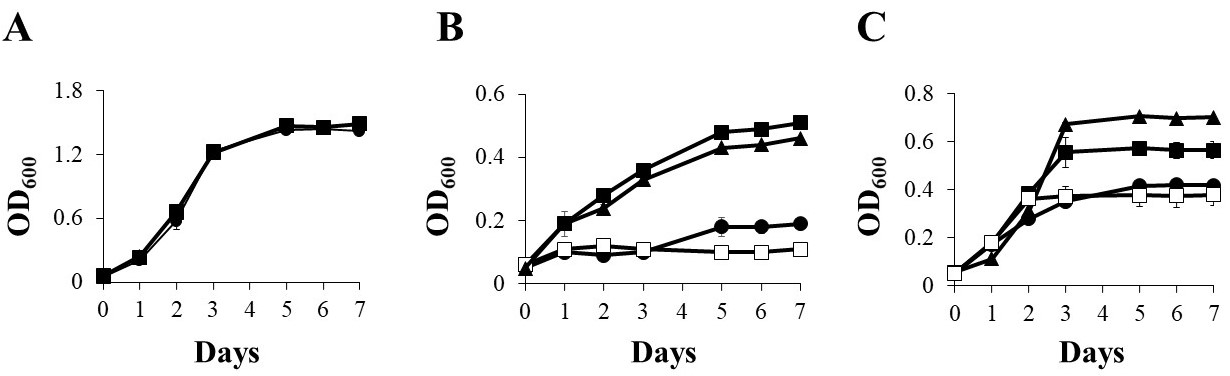
\includegraphics[height=5cm]{Images/Figure1.jpg}
\caption{Growth of {\em B. diazoefficiens} 110spc4 in Cu limitation (Cu-L) (circle), Cu standard (Cu-S) (square) and
high Cu (Cu-H) (triangle) BVMN media under oxic (A), anoxic (B) and microoxic (C) conditions. In (B,C),
growth in the Cu-S BVM medium was also included (white square). Error bars represent standard error between
triplicates, and where not visible, these were smaller than the symbols}
\end{figure}
\begin{figure}[h!]
\centering
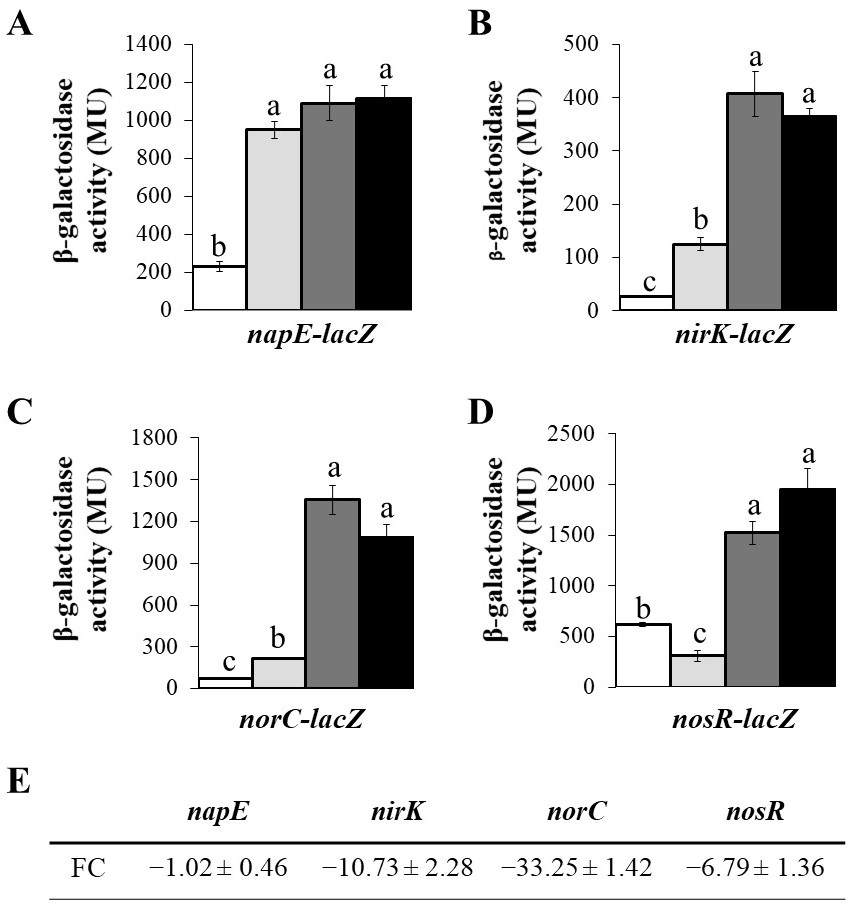
\includegraphics[height=13cm]{Images/Figure2 (2).jpg}
\caption{Transcriptional expression of denitrification genes monitored as $\beta$galactosidase activity
from {\em napE-lacZ} (A), {\em nirK-lacZ} (B), {\em norC-lacZ} (C) and {\em nosR-lacZ} (D) fusions chromosomally integrated
in {\em B. diazoefficiens} 110spc4 grown aerobically in Cu-S (white bars) and microaerobically in Cu-L (light
grey bars), Cu-S (dark grey bars) and Cu-H (black bars) BVMN media for 3 days. A post-hoc Tukey
HSD test at p minor to 0.05 was applied in (A–D); same lower-case letters in each figure indicate that
values are not statistically different. (E) Expression changes of {\em napE}, {\em nirK}, {\em norC} and {\em nosR} genes in
{\em B. diazoefficiens} 110spc4 grown microaerobically in Cu-L compared with Cu-S measured by qRT-PCR.
Data expressed as Miller Units (MU) and Fold Change (FC) are means with standard deviation from
at least three independent cultures assayed in triplicate.}
\end{figure}

\section{Conclusions}
The main goal of the present work was to investigate the influence of Cu on denitrification
in the soybean endosymbiont {\em B. diazoefficiens}. Taken together, our results suggest that
Cu may
act as an essential factor in the regulation of the denitrification gene expression. Therefore, Cu could be involved in the denitrification regulatory network and
not only acts as a mere enzymatic cofactor of the Cu-dependent enzymes, but also as an
important regulatory signal of this process.

\bibliographystyle{unsrt}
\bibliography{references.bib}

\end{document}  